\documentclass[]{article}
\usepackage{graphicx}
\usepackage{hyperref}
\usepackage{amsmath}
\usepackage{caption}

%opening
\title{Vacuum Science and the Influence of Vacuum Conditions on Thin Film Growth}
\author{Gunther T\"urk, Jonas Lehnen}

\begin{document}

\maketitle
\tableofcontents
\begin{abstract}
In this experiment our main goal was to learn how one applies the kinetic gas theory at the example of a vacuum chamber. Especially how one is able to create high vacuum by turbo pumping the chamber and even further decrease the pressure by baking it. 

Write here, what we did and learned.
\end{abstract}

\section{Theorie}
\subsection{Kinetic Gas Theory}
In kinetic gas theory we assume a gas to consist of many microscopic spheres which don't interact with each other and take negligible volume in a container. The particles can move freely and spread homogeneously in a given container. When they crash onto the container walls they exert a force on these, we can measure as pressure. 
\[ p=F/A \]
It is measured in [Pa] or [bar].
\[ [Pa]=N/m^{2}     \qquad  1bar=10^{5}Pa		 \]
What we can measure as temperature is caused by the movement of the particles in the gas. So it has to be related to the kinetic energy, what explains why the pressure on the walls rises, if we increase the temperature. From experiments done in the 17th and 18th century we know the state equation for an ideal gas
\[ pV=nk_{B} T\]
 where $k_{B}\approx1,38J/K$ is the Boltzmann constant and temperature is measured in Kelvin.We assume for our purpose that all particles are incompressible hard spheres and that there are no frictional forces between the particles and the walls. Because the particle speeds are distributed isotropically there are $1/3N$ particles moving along each axis. For simplicity we consider a particle moving along the x-Axis with the velocity $v_{x}$. Initially it has the momentum $p_{x}=v_{x}*m$. After an elastic collision with a wall its momentum is $-p_{x}$, so the momentum change is $\Delta p_{x}=2p_{x}$. We can calculate the force on the wall by multiplying the momentum change of each collision with the ammount of collisions per time interval. In a box with surface A and length $ds=v*dt$ there are \[ N=\frac{N}{V}A *v* dt \] particles of which 1/6 is moving in x-direction. So the total momentum transfer is \[ \Delta p_{i}=\frac{2N* A* v* dt*m* v}{6V} \]. For the force on the wall we get \[ F=\frac{dp}{dt}=\frac{ANmv^{2}}{3V} \rightarrow p=\frac{Nmv^{2}}{3V} \Leftrightarrow p=\frac{N*E_{kin}}{3V}\] Comparing this equation to the ideal gas law gives us that \[ v^{2}=\frac{3k_{b}T}{m_{p}} \] 
 Assuming we have a canonical ensemble of gas molecules we can conclude that the distribution of particle speeds can be described by a Maxwell-Boltzmann-statistic. \[ f(v)=\frac{m^{\frac{3}{2}}}{2\pi k T} 4\pi v^{2} e^{\frac{-mv^{2}}{2kT}} \] Now we can calculate the expectation value for the speed $<v>$ and also $\sigma_{v}$
 \[<v>=\int_{0}^{\infty}vf(v)dv=\sqrt{\frac{8kT}{\pi m}}  \]
 \[ \sqrt{<v^{2}>}=\int_{0}^{\infty}v^{2}f(v)dv=\sqrt{\frac{3kT}{\pi m}}  \]
 The second result is consistent with the speed we derived earlier with simple thoughts about pressure. We can easily see that lighter particles move a lot faster than heavier ones. 
 \paragraph{Example}
 \mbox{}\\
 If we have an $H_{2}O$ molecule at room temperature (300K), we can calculate its thermal speed and energy.\[ 
 v=\sqrt{\frac{3kT}{\pi m}}=363\frac{m}{s} \]
 \[ E_{thermal}=\frac{1}{2}mv^{2}=1.09*10^{-22}J \]
\\\\\\\\
\subsubsection{Mean free path}\
The mean free path of a particle is described as the length after which $e^{-1}$ have not hit another particle yet. We can estimate the mean free path $\lambda$ in a gas if we know the total cross section $\sigma$  of a particle. The mean free path multiplied with the cross section gives us the effective volume the particle has covered. If in average a particle has then hit another particle the product of the covered volume with the particle density should be one.\[\lambda \sigma *\frac{N}{V}=1 \Leftrightarrow \lambda=\frac{V}{N\sigma}  \]

\paragraph{Example}\mbox{}\\
We will calculate the mean free path of nitrogen ($N_{2}$) molecules in atmospheric pressure and at $10^{9}mbar$. Nitrogen $N_{2}$ has an atomic radius of $r = 155 pm$ (Van der Waals radius). \[\sigma_{N_{2}}=\pi r^{2}=7.55*10^{-20}m^{2} \]\[ \frac{V}{N}=\frac{k_{b}T}{p} \Rightarrow \lambda_{Atomsph.}=54.88\:nm   \quad ;\lambda_{10^{-9}mbar}=5.5*10^{6}m \]


\subsection{Desorption}
Molecules and Atoms can stick to a surface e.g. the walls of our vacuum chamber, through dipole or van der Waals forces and covalent linkage. The process of getting them off again is called desorption. For desorption we need to add kinetic energy in form of heat to the particle until the $E_{kin}>E_{des}$. The desorption energy vary in different kinds of molecules and atoms. From Boltzmann-statistics we know that there are $\Delta n=ne^{\frac{-D_{des}}{RT}}$ particles with a high enough kinetic energy to leave the surface again. Because our walls are in a heat bath with the lab they don't loose heat so that the temperature stays constant so that there are always particles with enough energy to desorp from the walls. The Polanyi-Wigner equation then tells us what the rate of desorption in our chamber is, with $\nu=\frac{kT}{h}$ being the oscillation frequency of the molecules.\[ j_{des}=\frac{dn}{dt}=-\nu n e^{-\frac{E_{des}}{RT}} \] 
\begin{figure}[h]
	\includegraphics[width=0.7\linewidth]{"Plots/Polanyi Wigner"}
	\label{fig:polanyi}
	\caption{Polanyi Wigner equation for different temperatures}
\end{figure}


\subsection{Pumps}
We use different pumps to produce a high vacuum for the different pressure regimes. The pre pump is used to get to a low enough pressure to use the turbo pump which gets us to a very high vacuum.

\subsubsection{Pre Pump}
The pre pump (Fig. \ref{fig:prepump}) works by changing the volume in a pumping chamber while opening and closing 2 valves. During the inlet phase the valve towards the vacuum is open, and the one towards the atmosphere is closed, while the volume in the pump is increased. This is reversed during the outlet stage.

\begin{figure}[h]
	
	\centering
	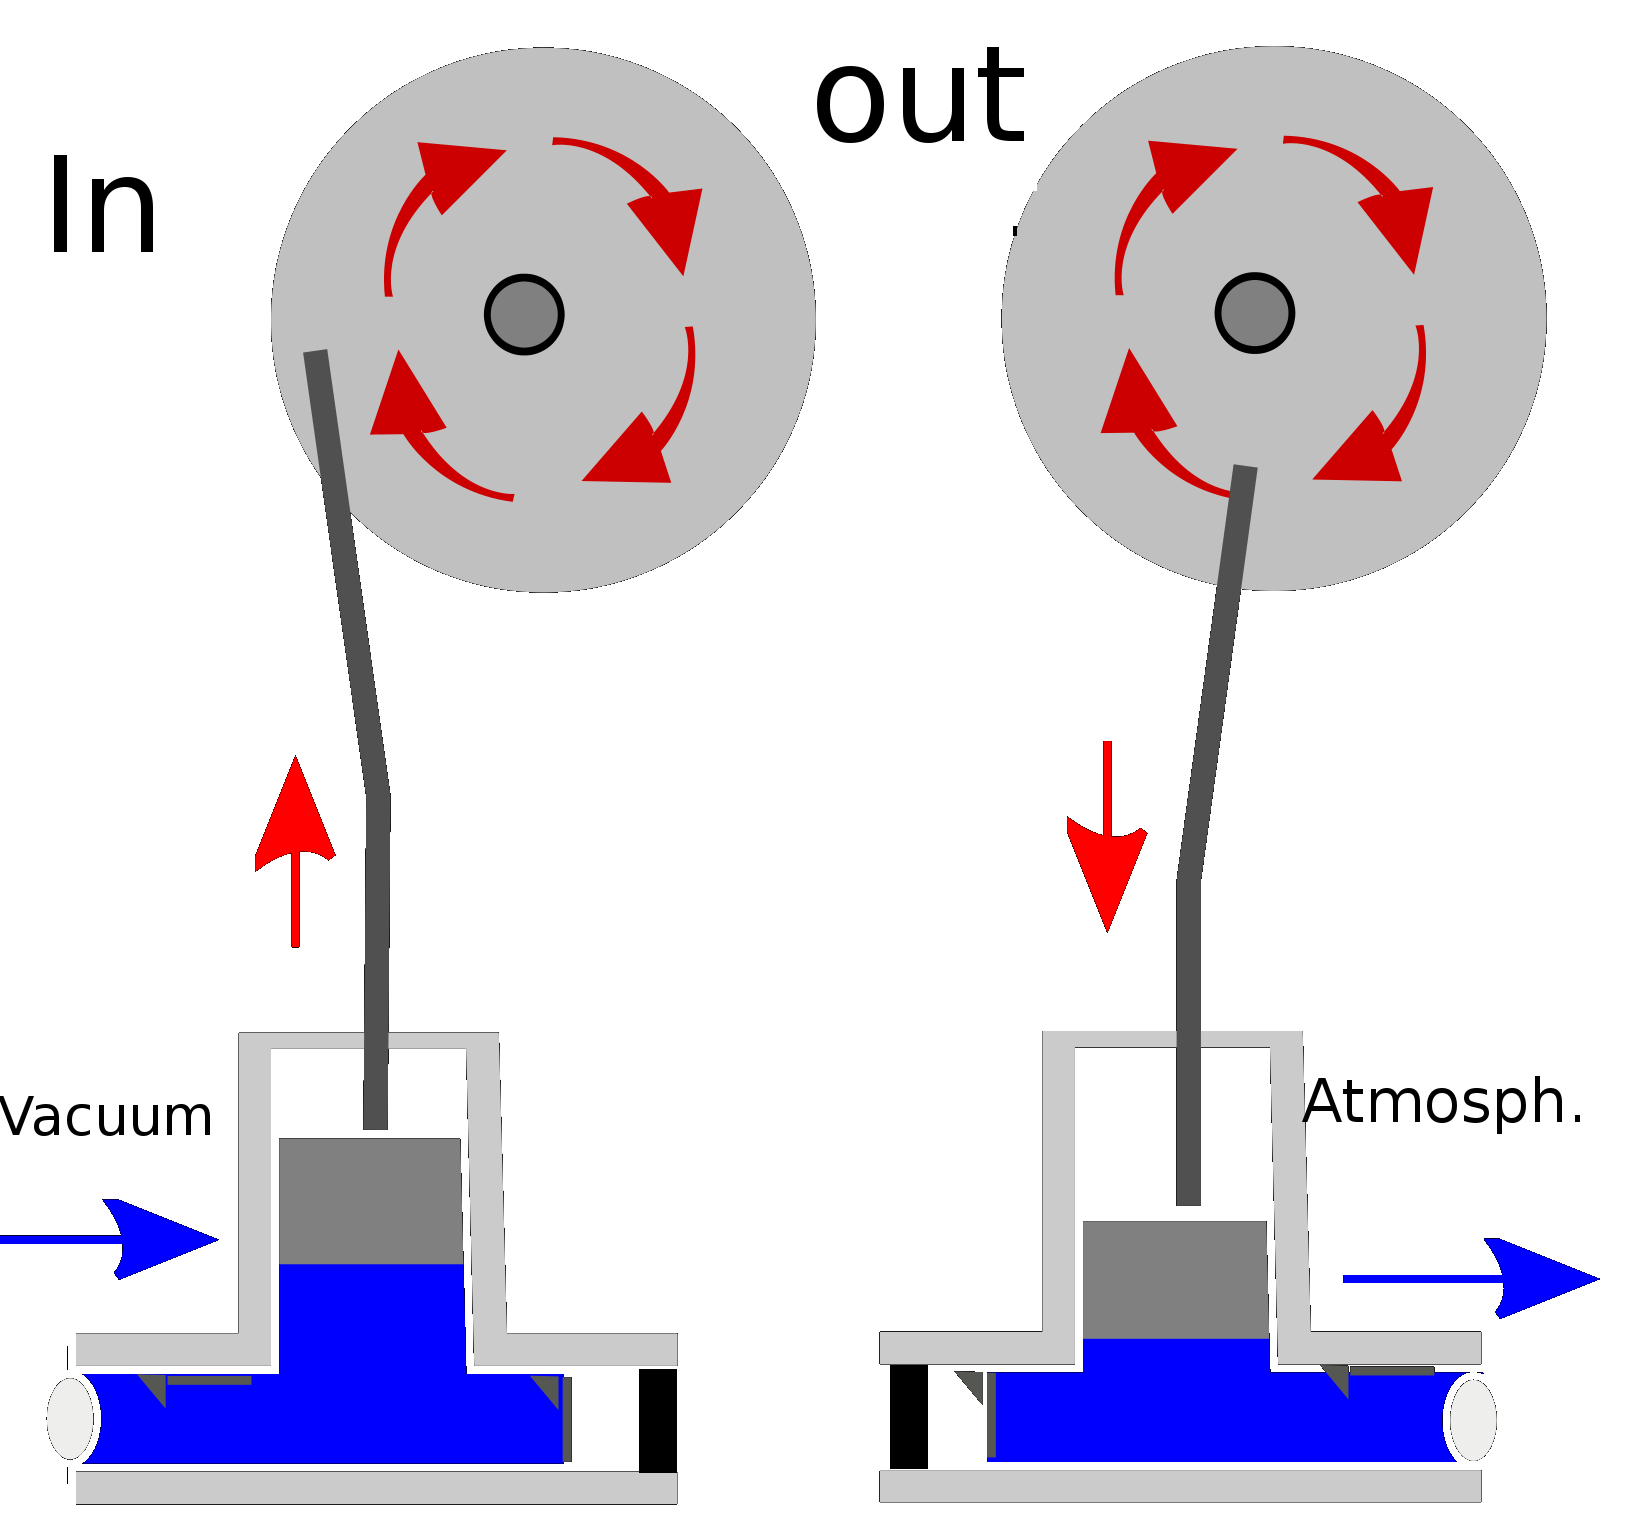
\includegraphics[width=0.5\linewidth]{Bilder/pump}
	
	\caption{Schematic representation of a pump}
	\label{fig:prepump}
\end{figure}

The pressure limit we can reach with the pre pump alone is on the one hand caused by leaks of the valves and the piston. On the other hand there is a pressure limit even with perfect valves by the air ($V_{0} $) at atmospheric pressure which remains in the cylinder at the outlet stage . With isotherm expansion in the cylinder we can calculate this minimum pressure to be: \[ p_{min}=p_{Atmosph.}\frac{V_{0}}{V_{max}} \]

\subsubsection{Turbo Pump}
Different from the pre pump which works by producing a pressure gradient between two chambers, a turbo pump works through the principle of momentum transfer. Atoms in a chamber don't bounce elastically of the walls but stick to them through adsorption for a short amount of time, so it is possible to accelerate them with spinning rotors in the turbo pump and push the atoms to the outlet. This only works if the mean free path of a particle is lager than the distance between the rotor blades, which is why we connect the outlet of the turbo, to the pre pump. Our turbo pump is able to evacuate 300 litres of gas per minute.

Considering the effective amount of volume getting pumped out $S_{eff}$ and an empty chamber, we can calculate how many atoms per time $\dot{N}$ are getting desorbed from the wall.

\[ \dot{N}=\frac{q_{pV}}{k_BT}= \frac{p\dot{V}}{k_BT} \: , \quad \dot{V}=S_{eff}= \frac{V_{chamber}}{\Delta t}ln \frac{p_0}{p_1} \]

\paragraph{Example}\mbox{}\\
Also considering that the pressure is nearly constant, so we can use the mean value $p=\frac{p_0+p_1}{2}$. A pumping process with $t_0=1250s,\: p_0=10^{-5}mbar$ and $t_1=2750s,\: p_0=5\cdot 10^{-6}mbar$ for a chamber with 30l volume and $T=293K$ results in $\dot{N}=25.7\cdot 10^{6} \frac{1}{s}$. This is analogue to $1.24\cdot 10^{-15} \frac{g}{s}$ of air getting pumped out (Mass of air $29 \frac{g}{mol}$).
\label{dn}


\subsection{Thin Films}
These films are layers of material with a thickness between a few atomic radii to several micrometers, which are grown on a substrate for mechanical support. But why do we want to create thin films?

The main usage of thin films is to create a layer of the targets material which can result a reduction of the refractive index. This is used to reduce the amount of reflected light on lenses for optical instruments and glasses. But also the opposite is possible. For example, by sputtering copper the resulting very clean and even layer can reflect nearly all light, see Fig. \ref{fig:sample}. 

Both variation are used in solar panels. The top layer should be able transmit almost every photon, so the photovoltaic effect can create electrons and thereby a current. The bottom layer should reflect almost every photon, that hasn't been absorbed yet.

\subsection{Sputtering}
Sputtering is a mechanical process used to create thin films, at which we bombard a target with ions to dissociate single atoms from the target and subsequently deposit them on the substrate. We enrich our vacuum chamber with Ar and shoot an electron ray into it. The electrons ionise the Ar atoms, what leads to even more electrons emitted in the chamber. If there is enough space between the cathode and the anode for electrons to hit other Ar Atoms and the concentration of Ar is high enough they will form a plasma. To accelerate the Ar atoms towards the target we apply a DC voltage that also accelerates the electrons further what helps with the ionisation. It is possible to use a magnetic field to contain the plasma in a small area around the target. The free Atoms in the chamber then will adsorb onto the surface of our substrate. Because sputtering is a purely mechanical process, we can sputter different metal alloys and keep the stoichiometry on our thin layer.


\subsection{Flow}
The phenomena of flow occurs everywhere we have moved particles in a given space. The common example is a tube with diameter d where molecules are streaming through. Literature differentiates between three types depending on the pressure and determinable by the Knudsen number Kn.
\[ 0.5 > Kn := \frac{\lambda}{d} > 0.01 \qquad for\: transitional\: flow\]
At low pressures and high Kn it's called molecular flow. At this point collisions between the particles are very uncommon and only the collisions with the wall are changing the movement. This results in a zigzag trajectory along the tube. For higher pressure it gets into the transitional flow where both collisions are equally common. Then for low Knudsen numbers the viscous flow is relevant. In this connection one differentiates again between laminar and turbulent flow depending to the particles velocity v in the tube.

\subsubsection{Laminar}
Crucial for this distinction is the Reynolds number Re. Besides v and d, Re depends on the density $\rho$ and the viscosity $\eta$ of the particle stream. Is its value below 2300 we can speak about pure laminar flow. Thereby the particles moving in the center of the tube are faster than the ones further outside due to their higher chance of hitting the wall and getting their momentum changed.
\[ Re:= \frac{\rho}{\eta} v d\]

\subsubsection{Turbulent}
If the Reynolds number is above 4000 turbulent flow is present. Thereby we can observe turbulences created by the stronger decelerated particles near the wall. They will nearly stick to the wall which forces the next particle layer onto the next part of the wall. While the particles in the center are less affected due to their distance. With longer tubes this deceleration starting at the wall can proceed into every layer and you'll observe laminar flow again. \\
For $2300 < Re < 4000$ some turbulences will occasionally occur.


\subsection{Gauges}
There are 3 different kinds of pressure gauges in our vacuum chamber, each designed to work best at different pressures. While it is possible to change technical parameters for every gauge the mode of operation of each gauge suits it best for a specific regime.

\subsubsection[Capacitive]{Capacitative Pressure Gauge}
The capacitive pressure gauge is basically a plate capacitor with a insulator in between. One plate is connected to the chamber, so that the pressure difference will push the plates together. That causes the conductivity to increase what we then can measure. It can be used at higher pressures. 

\subsubsection[Pirani]{Pirani Pressure Gauge}
A pirani gauge consists of a metal filament (usually platinum) connected to an electrical circuit. The filament is heated when the current flows through. At every collision with a gas molecule it gives heat to the molecule, what causes the temperature of the filament to drop. The rate of molecules hitting the filament is proportional to the amount of molecules in the chamber, so cooling of the filament slows down with sinking pressures. Because the resistance of the filament rises with temperature we can use the measurement of it to get a pressure reading from our gauge. It may be used at pressures between $0.5\ mbar$ to $10^{-3}mbar$.

\subsubsection[Penning]{Penning Pressure Gauge}
A penning gauge is made out of a cyllindric metal cage, serving as the cathode and a inner filament which serves as the anode. In a right angle to the plane of the field lines is a magnetic field, causing electrons emitted from the cathode to move in long spiral orbits towards the anode. In this process they ionise the molecules left in the chamber what causes cascades of electrons emitted to the anode, even an very low pressures. The current decreases with lower pressure, since frequency of collisions as well as cascade intensity both decrease. It can be used for pressures between $10^{-2}mbar$ to $10^{-7}mbar$.


\subsection{Questions}
\subsubsection{Day1}
\begin{itemize}  
	\item What causes the limit on the pressure one can reach with the pre-pump alone? $\surd$
	\item  Calculate the mean free path of a nitrogen (N2) molecule in atmospheric pressure and at $1 \cdot 10^{−9}$ mbar $\surd ?$
	\item Based on the data from section 5.3, how much gas is desorped from the walls after the turbo reaches full speed? Hint: Consider the data over the time period after the turbo reaches speed. This is the pressure drop in a fixed time. The volume of the chamber is 30 litres and you can assume the chamber is at a constant temperature of 293K. The mass of air is approximately 29g/mol.
	 

	\item What is the purpose of baking out a chamber? $\surd$
	\item What is the thermal energy at room temperature and the corresponding thermal speed of a water molecule (H2O)? $\surd$
\end{itemize}

\subsubsection{Day2}
\begin{itemize}
	 \item Can you name some properties which might arise due to scaling down the thickness of a sample?
	  \item How have the elemental peaks changed from the spectra of the first day? What can you say about the baking process? How will the baking process affect the quality of the samples being grown? 
	  \item Why does the pressure oscillate with clear periods of increasing and decreasing pressures during baking? $\surd$
	  \item What happens to the plasma as you increase the power being applied to the cathode? $\surd$
	\item Why do we pre-sputter the target before deposition? $\surd$ 
	\item  Plot the Polanyi-Wigner equation as a function of desorption energy for an ensemble of $5.35 \cdot 10^{13}$ particles for $T_w$ = 300K, 500K, 800K, 1000K for Edes between 0 and 60 kJ/mol (universal gas constant 8.31 J/mol). Scale the y-axis to $10^{13}$ as a maximum. $\surd$
	
\end{itemize}



\newpage
\section{Experiment}
As already mentioned the main task of the experiment was to learn how the vacuum chamber works and being able to operate it. 

We were allowed to operate a vacuum chamber with a volume of 30 litres. The inside is reachable by the main window which is hold by eight bolts and a copper seal. The sputtering targets are at the bottom while a rotatable disk, where the sample was placed, is in the center. This one is operate-able from the outside. At the backside the pressure gauges are connected. 
The chamber itself was connected to a turbo pump, which itself was connected to a valve with electric controls as well a brass cap for the venting. Behind the turbo pump the pre-pump with a 25mm diameter tubing was placed. Above the pumping systems is the mass spectrometer with its filament.

\subsection{Pre-Pumping}
The first task of Day 1 was to confirm the equations for flow resistance R and conductance C, \cite[Page 91]{VacuumHandbook}. 
\[ \quad Series \: Connection: \quad
R = R_1 + R_2 + ...  \quad \frac{1}{C} = \frac{1}{C_1} + \frac{1}{C_2} + ... \]
\[ Parrallel \: Connection: \quad
C = C_1 + C_2 + ...  \quad \frac{1}{R} = \frac{1}{R_1} + \frac{1}{R_2} + ... \]

To do so we exchanged the tubes connecting pre-pump and the vacuum chamber. Our different tube diameters were 25mm and 40mm. With three measurements of the pressure change in time, each tube alone and once in series connection. With the data we are able to determine the effective pumping speed, see \cite[Page 93]{VacuumHandbook}, given by:
\[ \frac{1}{S_{eff}} = \frac{1}{S} + \frac{1}{C} \quad , \quad
S_{eff} = \frac{V}{\Delta t} \ln{ \frac{p_0}{p_1} } \]

From the second equation we get three different $S_{eff-i}$, where 1 stands for the 25mm diameter tube and 2 for the 40mm one. According to the first one, we now can calculate the real pumping speed and the conductances of both tubes. The real pumping speed S should be around 8 litres per minute.
\[ \frac{1}{S} = \frac{1}{S_{eff-1}} + \frac{1}{S_{eff-2}} -\frac{1}{S_{eff-12}} \quad , \quad
\frac{1}{C_i} = \frac{1}{S_{eff-12}} - \frac{1}{S_{eff-i}} \]

The results of those equations are: dersfydgxtfcx

\begin{figure}[!h]
\centering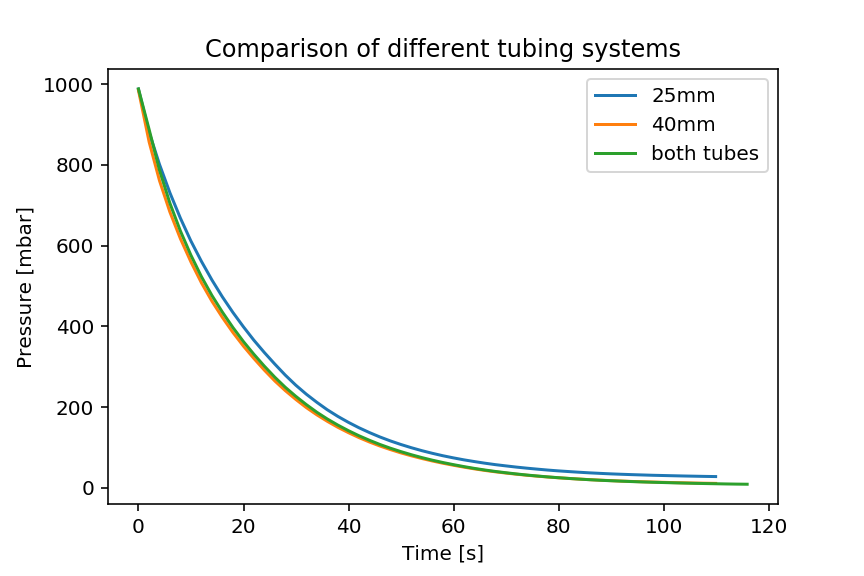
\includegraphics[width=.75\textwidth]{Plots/Comparison.png}
\caption{Pressure change in time for every tube set-up.}
\label{fig::comparison}
\end{figure}


\subsection{Turbo Pumping}
After loading a sample into the chamber we started the pre pump and at $10^{-1}mbar$ the turbo pump while measuring the pressure with different gauges. You can see in Fig \ref{fig:pumpingpressure} each gauge is most accurate for its certain pressure regime.
As already shown in the pre-pump graphics the pre-pump lowers the pressure down to less than 10m bar within 100s and also could keep on lowering it, as you can see at the full range sensor. To speed the pumping process up, the turbo pump gets activated. As you can see the pressure dropped dramatically fast until the chamber was nearly empty. Now only the newly desorbed are getting pumped out. Until 1111s in the measurement the turbo was running at 30k rpm with a driving power of 4W. Then we recognised that this was only 50\% of its power and increased it to 60k rpm and 12W. With these settings we went on with the following tasks and measurements.

\begin{figure}[!h]
	\centering
	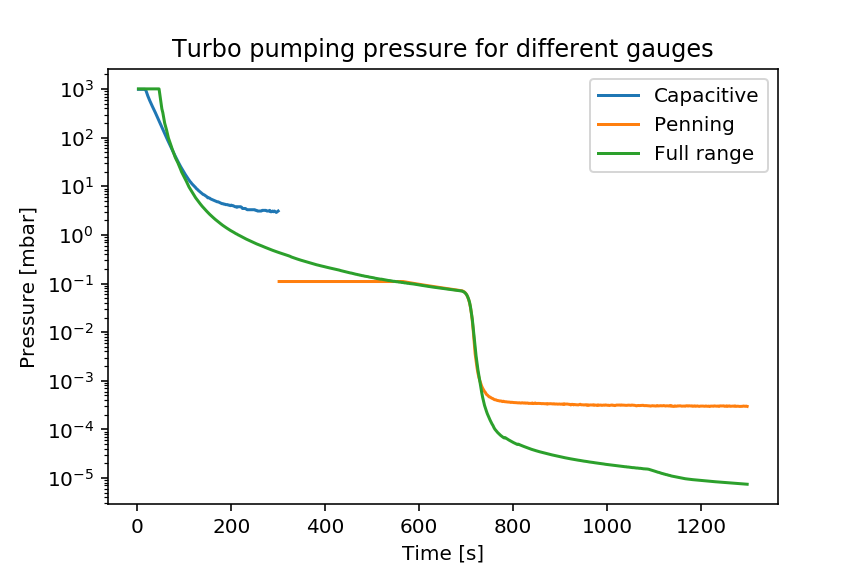
\includegraphics[width=0.7\linewidth]{Plots/PumpingPressure}
	\caption{Pump down pressure from different gauges}
	\label{fig:pumpingpressure}
\end{figure}

Now you can do the same exemplary calculation as in \ref{dn} for the time values $t_0=1200s, \: t_1=1600$ and we get $ \dot{m} = 9.4\cdot10^{-16} \frac{g}{s}$. 
As you can see, this value is very small. But this is what we've expected by the first calculation and that the amount of adsorbed atoms on the wall cannot be in usual dimensions we are thinking in.git add *



\subsection{Mass Spectrometer}
The next task was to look at the elements in our vacuum chamber. We want to know how their amount changes with the baking process. We are especially looking for the atoms most common in our standard air:

\begin{table}[h]
\centering
\begin{tabular}{lcccccc}
Elements & $H_2$ & $H_2O$ & $N_2$ & $O_2$ & $Ar$ & $CO_2$ \\
Molar Mass & 2 & 18 & 28 & 32 & 40 & 44 \\
\end{tabular} 
\end{table}

Turning on the mass spectrometer below a pressure of $10^{-6} mbar$ ensures that it won't break due to too many atoms around. They would all be ionised and the current we are measuring would be too high for the sensitive MS. Setting the MS in the range from 1 to 50 amu we now can compare our two measurements. For each atomic mass measure time of 10s was given. Thereby we want to ensure that our peaks are sharp and clearly visible. The individual graphics are shown in \ref{MS Plots}.

\begin{figure}[h]
\centering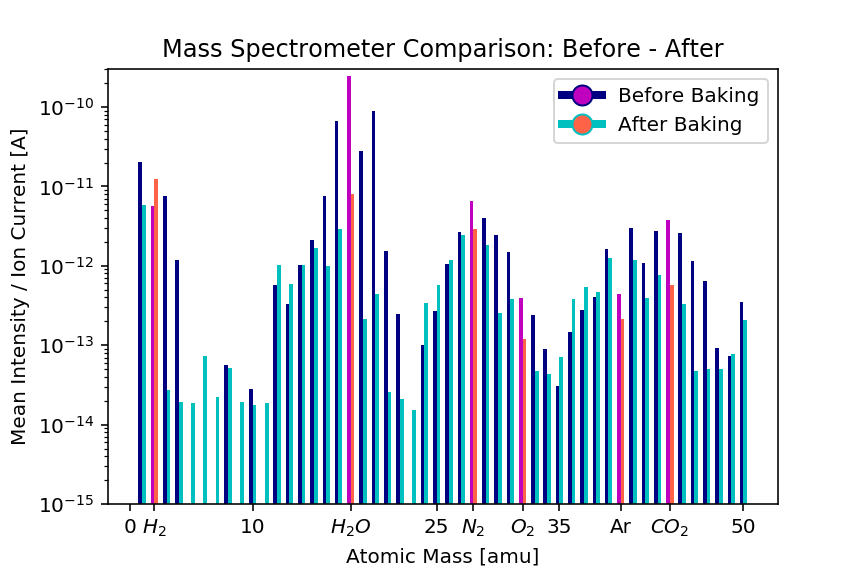
\includegraphics[width=1\textwidth]{Plots/BeforeAfter.png}
\caption{Results of the mass spectrometer before and after the baking process.}
\label{fig::BeforeAfter}
\end{figure}

The plot shows exactly what we wanted to achieve. The intensity of most molar masses dropped after baking. Looking at the main peaks $N_2$ and $CO_2$ dropped by around half of a magnitude,  $H_2O$ dropped even by a whole magnitude. The $H_2$ on the other hand increased for a little bit.

With less pressure and therefore less atoms in the vacuum chamber the mean intensity of the bars decreased. 

\subsection{Baking}
This process of baking is pretty self-explanatory. While the turbo pump was active, we wrapped heat belts around the vacuum chamber and covered them with blankets to decrease the loss of thermal energy to the surrounding air. Before turning them on, to heat up the chamber for around 9 hours, we had to remove all heat sensitive components like the mass spectrometer and covered the windows with silver foil to prevent a to large heat difference, which could cause them to break and negate the whole process of creating a vacuum.
The longer the heating time is the better the vacuum can get. By heating you allow the adsorbed atoms of the inside wall get free and pumped out. 
For the second mass spectrometer we need the chamber to cool down to room temperature, therefore the baking ended again 9 hours before we arrived for the Day 2.

\begin{figure}[h]
\centering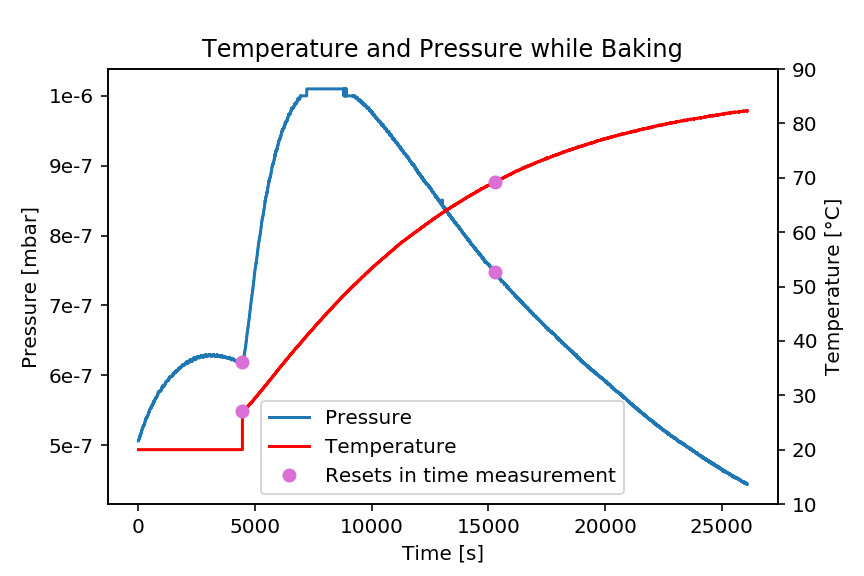
\includegraphics[width=.75\textwidth]{Plots/Baking.png}
\caption{Change in pressure for the first part of the baking process. Due to software problems this is the only data.}
\label{fig::baking}
\end{figure}

As you can see in Fig.\ref{fig::baking} the temperature didn't increase in the first part of the measurement. This is caused by the positioning of the thermometer, which was placed in the center of the chamber. Less atoms means that the rising energy from the wall needs it time to get transferred. 
The sensor only kicks in for higher temperature that room temperature, for this reason you can see the jump from 20°C to the actual value. This could also be the reason why the software decided to restart the time measurement at this moment. 

Looking at the second measurement, the middle part in Fig.\ref{fig::baking}, the pressure increases rapidly before falling down again. This is the effect of the adsorbed atoms coming free and increase the pressure. If the rate of them coming free is then less than the rate of them getting pumped out, the pressure will decrease again. This process should happen many times, depending on the different desorption energies of the different molecules. 
This is already shown in the first part of the measurement by the first peak in the pressure change. The little bump before the crossing of temperature and pressure seems to be caused by some kind of noise, because it was only there for about one measure point (Appendix Fig.\ref{fig::bump}).

point of baking, probe quality. The whole reason of baking is not only to create a better vacuum for its own sake, but to remove as many unwanted atoms as fast as possible. Due to Boltzmann statistics we could achieve the same pressure within a longer time, because in an ensemble there will always be one atom with the necessary energy to leave the wall. Baking reduces the waiting time by increasing the energy of the adsorbed atoms.
With less pressure and atoms within the chamber there are less atoms which could affect the quality of our thin film growth. That means the quality of our sample will increase automatically with better vacuum.

The results of our baking were as expected but still impressive. We started with a pressure of $5.10 \cdot 10^{-7} mbar$ and at the beginning of Day 2 we already fell to $3.86 \cdot 10^{-8} mbar $. This decrease of one magnitude after only one day is the reason other chambers are getting baked for a week, if you need the lower pressure.

\subsection{Film growth}
After baking the chamber over night we were ready to sputter our target and grow a film on the substrate. 

\subsubsection{Pre Sputtering}
At first we had to pre sputter our target for 5 minutes to remove any unwanted particles which adsorbed onto its surface, to prevent them from desorping onto our substrate later on when the substrate is above the target. Pre sputtering reduces the amount of impurities in our thin film and improves the quality of the sample.  We slowly opened the valve of the argon and adjusted the valve until the pressure in the chamber would stay constant at $3*10^{.2}mbar$ . When turning on the DC voltage we could immediately see a plasma burning.

\subsubsection{Plasma}
The plasma burned in a cone shape above the target with a light blue color. After the pre sputtering was done we measured an I-V-curve for the plasma (Fig \ref{fig:ivcurve}) and observed how it was burning. At low currents up to $3mA$ the plasma was flickering. At higher currents it started to burn stable and we saw a linear relation between I and V what tells us that the plasma at higher currents behaves like a ohmic resistor. Because we connected our target to a current generator a voltage was building up until enough electrons were emitted to ionise the argon and subsequently form a plasma. At low currents there are arriving much more argon ions at the cathode than electrons are emitted from our source. That causes the the voltage to drop and the plasma stops burning. With higher currents we can compensate the ions dragged to the cathode and keep up the voltage so the plasma burns stable.

\begin{figure}
	\centering
	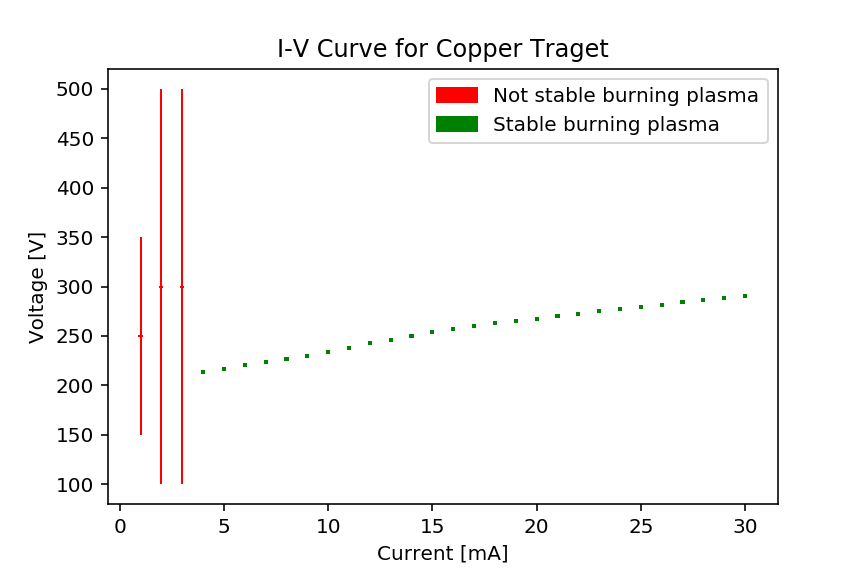
\includegraphics[width=1\linewidth]{Plots/IVcurve}
	\caption{For low currents we can see the voltage jumping around in a wide realm. For higher currents we see a linear increase in voltage}
	\label{fig:ivcurve}
\end{figure}

\subsubsection{Film Growth}
To finally grow our thin film we adjusted the current to a stable regime and moved our substrate into the plasma for 15 minutes. We can see a shiny layer of copper on the side facing the plasma.  

\begin{figure}
	\centering
	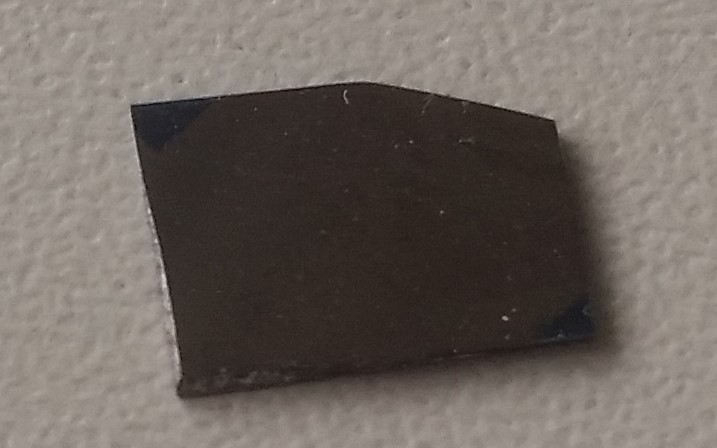
\includegraphics[width=0.7\linewidth]{Bilder/sample}
	\caption{A picture of our sample. There is no copper where the substrate was glued to the holder}
	\label{fig:sample}
\end{figure}
	


\newpage

\section{Appendix}
\subsection{Pre-Pump Plots}
\label{Pre-Pump Plots}

\begin{figure}[!h]
\centering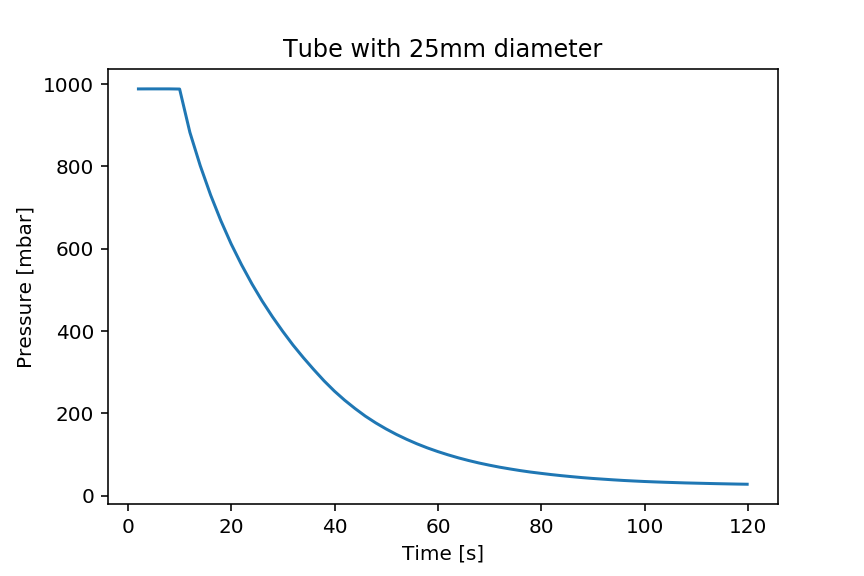
\includegraphics[width=.5\textwidth]{Plots/25mm.png}
\caption{The individual pressure change for the pre-pump and the tube with diameter 25mm.}
\label{fig::25mm}
\end{figure}

\begin{figure}[!h]
\centering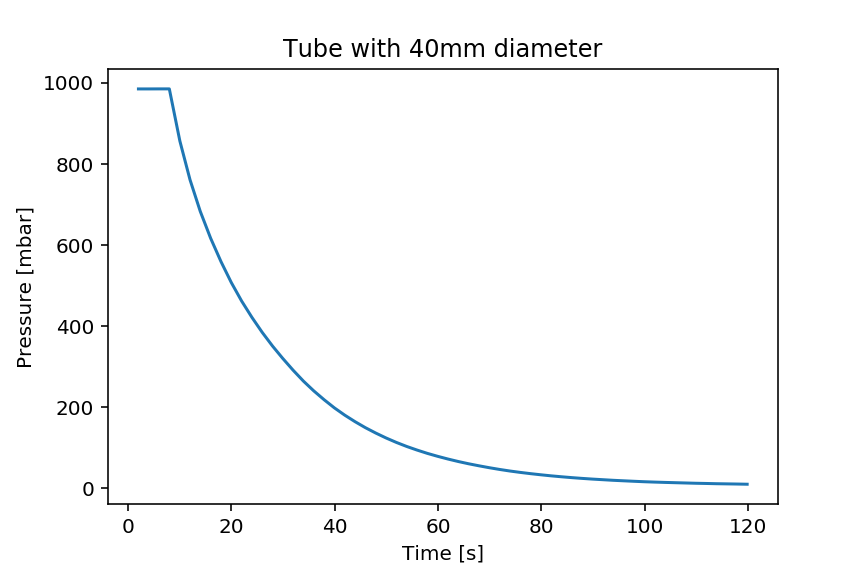
\includegraphics[width=.5\textwidth]{Plots/40mm.png}
\caption{The individual pressure change for the pre-pump and the tube with diameter 40mm.}
\label{fig::40mm}
\end{figure}

\begin{figure}[!h]
\centering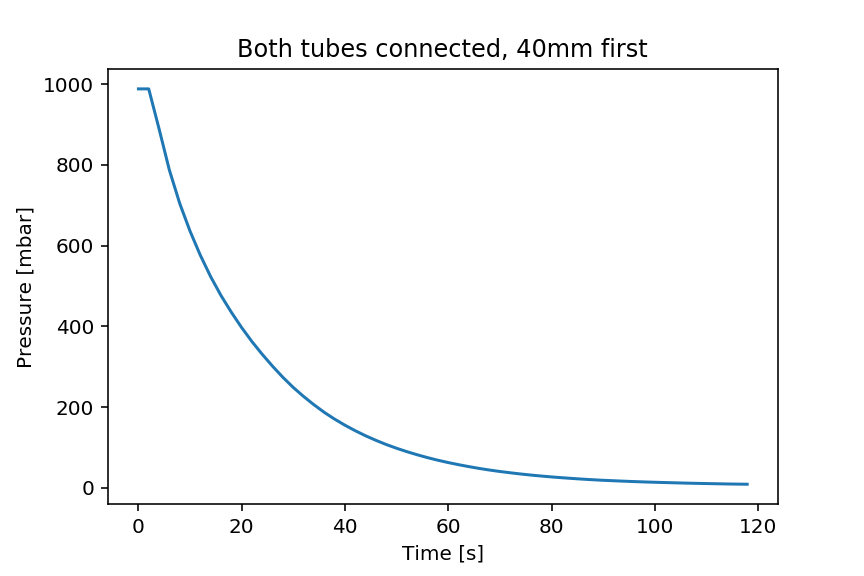
\includegraphics[width=.5\textwidth]{Plots/BothTubes.png}
\caption{The individual pressure change for the pre-pump and both tubes in series connection.}
\label{fig::BothTubes}
\end{figure}


\subsection{MS Plots}
\label{MS Plots}

\begin{figure}[!h]
\centering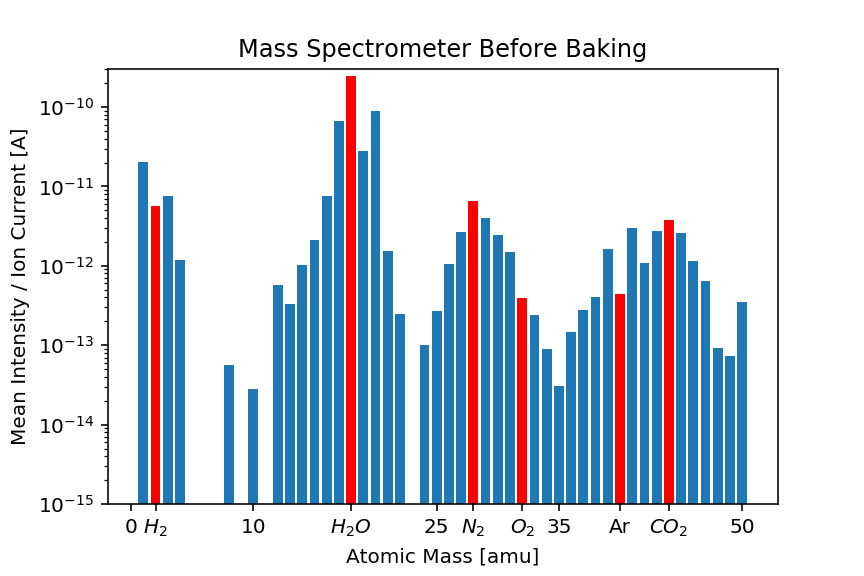
\includegraphics[width=.5\textwidth]{Plots/MSbefore.png}
\caption{Results of the mass spectrometer after baking.}
\label{fig::MSbefore}
\end{figure}

\begin{figure}[!h]
\centering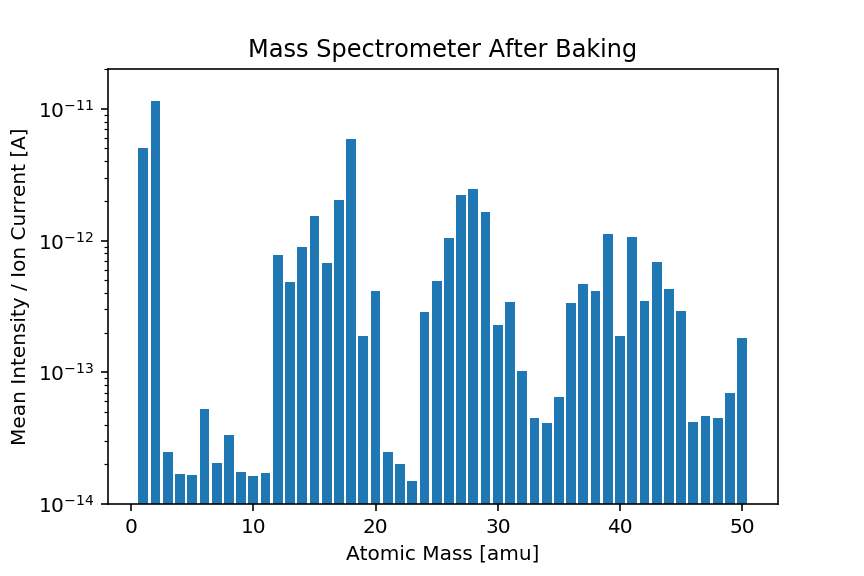
\includegraphics[width=.5\textwidth]{Plots/MSafter.png}
\caption{Results of the mass spectrometer after baking.}
\label{fig::MSafter}
\end{figure}

\subsection{Baking}
\begin{figure}[!h]
\centering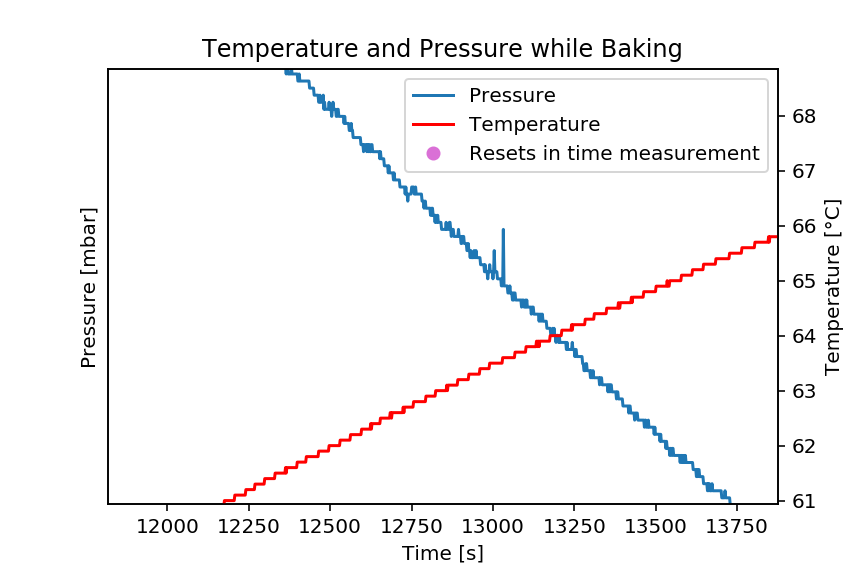
\includegraphics[width=.5\textwidth]{Plots/FluktuationBaking.png}
\caption{Zoom on the little bump which could have looked like another peak in the pressure.}
\label{fig::bump}
\end{figure}

\newpage
\begin{thebibliography}{9}

\bibitem{VacuumHandbook} Handbook of Vacuum Technology (Second Edition), edited by Karl Jousten, Wiley-VCH, 2016 (reprinted 2017), ISBN: 978-3-527-41338-6

\end{thebibliography}
\end{document}

